\newpage
\ifthenelse {\boolean{bachelor}}
{
	\section{Analysis}
	%\section{Analýza}
}
{
	\chapter{Analysis}
	%\chapter{Analyza}
}
Lorem ipsum dolor sit amet, consectetuer adipiscing elit, sed diam nonummy nibh euismod tincidunt ut laoreet dolore magna aliquam erat volutpat. Ut wisi enim ad minim veniam, quis nostrud exerci tation ullamcorper suscipit lobortis nisl ut aliquip ex ea commodo consequat. 
\ifthenelse {\boolean{bachelor}}
{
	\subsection{Subsection}
	%\subsection{Podčasť}
}
{
	\section{Subsection}
	%\section{Podčasť}
}
\label{label}
Lorem ipsum dolor sit amet, consectetuer adipiscing elit, sed diam nonummy nibh euismod tincidunt ut laoreet dolore magna aliquam erat volutpat. Ut wisi enim ad minim veniam, quis nostrud exerci tation ullamcorper suscipit lobortis nisl ut aliquip ex ea commodo consequat. Duis autem vel eum iriure dolor in hendrerit in vulputate velit esse molestie consequat, vel illum dolore eu feugiat nulla facilisis at vero eros et accumsan et iusto odio dignissim qui blandit praesent luptatum zzril delenit augue duis dolore te feugait nulla facilisi. Nam liber tempor cum soluta nobis eleifend option congue nihil imperdiet doming id quod mazim placerat facer possim assum. Typi non habent claritatem insitam; est usus legentis in iis qui facit eorum claritatem. Investigationes demonstraverunt lectores legere me lius quod ii legunt saepius. Claritas est etiam processus dynamicus, qui sequitur mutationem consuetudium lectorum. Mirum est notare quam littera gothica, quam nunc putamus parum claram, anteposuerit litterarum formas humanitatis per seacula quarta decima et quinta decima. Eodem modo typi, qui nunc nobis videntur parum clari, fiant sollemnes in futurum.
\begin{figure}[H]
\begin{center}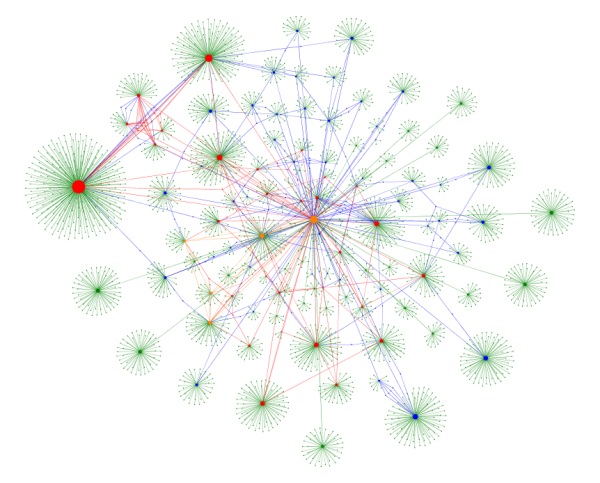
\includegraphics[scale=0.48]{figure}\end{center}
\caption[Name figure]{Name figure}\label{fig:figure}
\end{figure}
\subsection{Enumeration}
%\subsection{Číslovaný zoznam}
\begin{my_enumerate}
	\item {goal 1}
	\begin{my_enumerate}
		\item {goal 1.a}
		\item {goal 1.b}
	\end{my_enumerate}
	\item {goal 2}
	\item {goal 3}
\end{my_enumerate}
\subsection{Itemization}
%\subsection{Zoznam}
\begin{my_itemize}
	\item {item 1}
	\begin{my_itemize}
		\item {item 1.1}
		\item {item 1.2}
	\end{my_itemize}
	\item {item 2}
	\item {item 3}
\end{my_itemize}
\subsection{Citation}
%\subsection{Citácia}
Lorem ipsum dolor sit amet, consectetuer adipiscing elit, sed diam nonummy nibh euismod tincidunt ut laoreet dolore magna aliquam erat volutpat~\cite{1}.

\subsection{Labesl \& References}
%\subsection{Návestia \& Referencie}
See Section~\ref{lab:Examples}.

\subsection{Examples}
%\subsection{Príklady}
\label{lab:Examples}

\begin{lstlisting}[ language=html, caption={Example 1}, label={metrics_LOC},
	keywordstyle=\color{blue}\bfseries,
	ndkeywordstyle=\color{black}\bfseries,
	commentstyle=\color{red}\ttfamily,
	stringstyle=\color{green}\ttfamily,
	identifierstyle=\color{gray},
	backgroundcolor=\color{white}, 
	frame=single, 
	frameround=ffff,
	captionpos=b,
	basicstyle=\scriptsize
	]
<table class="metric_index">
	<tr>
		<th>Lines of code</th>
		<th>Value</th>
	</tr>
	<% if (filenum and modulenum) then %>
		<tr>
			<td class="name">Number of files</td>
			<td class="value"><%=filenum%></td>
		</tr>
		<tr>
			<td class="name">Number of modules</td>
			<td class="value"><%=modulenum%></td>
		</tr>
		<tr>
	<% end %>
	<tr>
		<td class="name">Lines Total</td>
		<td class="value"><%=LOC.lines%></td>
	</tr>
	<!--
							skryty zdrojovy kod
		podobne zobrazenie ostatnych metrik riadkov
	-->
</table>
\end{lstlisting}

\begin{lstlisting}[language=lua, caption={Názov}, label=metrics.pipe]
local parser  = require 'leg.parser'
local rules = require 'metrics.rules'
-- << skryty zdrojovy kod >> --
local capture_table = {}
grammar.pipe(LOC_capt.captures, AST_capt.captures)
grammar.pipe(block_capt.captures, LOC_capt.captures)
-- << viacero rovnakych volani s tabulkami captures inych modulov >> --
grammar.pipe(capture_table, cyclo_capt.captures)
local lua = lpeg.P(grammar.apply(parser.rules, rules.rules, capture_table))
local patt = lua / function(...) 
	return {...} 
end
local result = patt:match(code)[1]
\end{lstlisting}
